\documentclass[12pt,a4paper]{article}

\usepackage{geometry}
\geometry{a4paper, margin=2.5cm, top=3cm, headheight=20pt}

\usepackage{graphicx}
\usepackage{xeCJK}
\setCJKmainfont{PingFang TC} % macOS Standard Traditional Chinese

\usepackage{setspace}
\usepackage{titlesec}
\usepackage{amssymb}
\usepackage{hyperref}
\usepackage{enumitem}
\usepackage[table]{xcolor}
\usepackage{tcolorbox}
\usepackage{tabularx}
\usepackage{fancyhdr}
\usepackage{tocloft}

\setstretch{1.4}

% --- Header & Footer ---
\pagestyle{fancy}
\fancyhf{}
\rhead{\small \color{gray} 青年百億海外圓夢基金計畫 - 陳以珊}
\lhead{\small \color{gray} 海外翱翔組：AI 演算法遠征}
\rfoot{\thepage}

% --- Section Styles ---
\titleformat{\section}{\fontsize{16}{18}\bfseries\color[rgb]{0.1, 0.3, 0.6}}{\thesection}{1em}{}[\titlerule]
\titleformat{\subsection}{\fontsize{14}{16}\bfseries\color[rgb]{0.2, 0.4, 0.7}}{\thesubsection}{1em}{}
\titleformat{\subsubsection}{\fontsize{12}{14}\bfseries\color[rgb]{0.3, 0.5, 0.8}}{\thesubsubsection}{1em}{}

\hypersetup{
    colorlinks=true,
    linkcolor=blue,
    urlcolor=blue,
    pdftitle={青年百億海外圓夢基金計畫 - 陳以珊},
}

\begin{document}

% --- COVER PAGE ---
\begin{titlepage}
    \begin{center}
        \vspace*{1.5cm}
        {\huge \bfseries 青年百億海外圓夢基金計畫} \\
        \vspace{0.3cm}
        {\Large \bfseries 海外翱翔組 \quad 申請專案計畫書} \\
        \vspace{1cm}
        \rule{\textwidth}{1.5pt} \\
        \vspace{1.5cm}
        
        \begin{tcolorbox}[colback=white,colframe=blue!50!black,width=0.8\textwidth]
            \centering \Large \bfseries I-9-7 AI 演算法遠征 \\
            \vspace{0.2cm}
            \large Lambton College (加拿大) - AURORA 專案
        \end{tcolorbox}

        \vspace{2cm}

        \begin{tabularx}{0.6\textwidth}{rX}
            \textbf{申請人：} & 陳以珊（Yishan Chen） \\
            \textbf{目前單位：} & 上海交通大學 密西根學院 \\
            \textbf{主修專業：} & 電子與計算機工程學士 (ECE) \\
            \textbf{申請年度：} & 115 年度第二梯次 \\
            \textbf{見習領域：} & 人工智慧、大語言模型、自動化工程
        \end{tabularx}

        \vfill
        {\large 2026年3月}
    \end{center}
\end{titlepage}

\newpage

% --- TABLE OF CONTENTS ---
\renewcommand{\contentsname}{目錄}
\tableofcontents
\newpage

% --- EXECUTIVE SUMMARY ---
\section{計畫摘要 (Executive Summary)}

我是陳以珊，目前就讀於上海交通大學與密西根大學合辦之浦江國際學院（UM-SJTU Joint Institute）。在學期間，我始終致力於將前瞻的 AI 技術轉化為解決現實組織痛點的具體方案。

本計畫旨在前進加拿大 Lambton College 的「研究與創新（R\&I）」部門，參與其核心的 \textbf{AURORA (AI-driven Optimization \& Resource Automation)} 專案。透過我在大語言模型（LLM）、檢索增強生成（RAG）以及多智能體（Multi-Agent）架構上的實戰經驗，協助該機構優化其獎助金媒合與業務自動化流程。

\subsection{核心競爭力與亮點}
\begin{itemize}
    \item \textbf{工業級實戰指標}：在比特無限實習中，將工業意圖識別準確率從 \textbf{27\% 提升至 86\%}，並自動化審核流程，節省 \textbf{90\% 人工成本}。
    \item \textbf{獨立開發能力}：自主研發 \texttt{terny.ai} 科研機會匹配系統，高校識別準確率突破 \textbf{98\%}。
    \item \textbf{學術素養與倫理}：在百賢亞洲未來領袖獎學金（BXAI AFLSP）的支持下，深耕 AI 倫理（FASTER 原則），致力於開發負責任且具透明度的演算法。
\end{itemize}

\subsection{圓夢目標}
我希望透過為期 14 週的加拿大研究機構見習，不僅在技術維度深化對雲端部署與大模型工程的掌握，更要在國際化的工作環境中學習極致的倫理 AI 實踐。返台後，我將這套工業級 Pipeline 帶回國內，持續優化社會影響力專案，成為連結頂尖技術與本土應用的橋樑。

\newpage

\section{申請青年之學經歷深挖}

\subsection{學術背景與跨學科優勢}

\subsubsection{上海交通大學 - 密西根學院 (UM-SJTU JI)}
我就讀的密西根學院是全美與全中國頂尖工學院的深度合作結晶，採用全英文授課與密西根大學的教學體系。這段經歷賦予了我兩大關鍵能力：
\begin{enumerate}
    \item \textbf{嚴謹的計算與數據思維}：透過 \textit{Computational Methods} 與 \textit{Data Science} 課程，我建立了從原始數據到統計分析、再到模型預測的完整理論閉環。
    \item \textbf{國際化溝通與適應力}：在高壓且多元化的環境中，我學會了如何以英語進行高效的技術辯論與報告，這為我前往加拿大 Lambton College 奠定了溝通基礎。
\end{enumerate}

\subsubsection{核心專業課程與實踐}
\begin{itemize}
    \item \textbf{STAT 4060J: Computational Methods for Data Analysis} \\
    深入學習統計模擬（Monte Carlo）、優化算法（EM Algorithm）以及大規模數據集的數值分析。這為我後續處理 `OC22` 材料大數據集奠定了嚴謹的數學與算法基礎。
    \item \textbf{STAT 4710J: Data Science and Analytics using Python} \\
    掌握從 Exploratory Data Analysis (EDA) 到模型部署的完整 Python 生態鏈。在期末專案中，我獨立完成了房價預測模型，並在 RMSE 指標上達到班級領先。
    \item \textbf{ECE 3700J: Introduction to Computer Organization} \\
    學習計算機底層架構、流水線、指令集（ISA）。這使我能從「指令效率」的角度思考 AI 模型的推理優化，並能更好地理解 GPU 與硬體資源的分配邏輯。
    \item \textbf{VG 100/101: Introduction to Engineering \& Programming} \\
    啟蒙我的工程思維。在此課程中，我開發了首個自動化腳本，學會了如何透過程式碼解決重複性勞動。
\end{itemize}

\newpage

\subsubsection{國際交換：跨文化工作法與技術視野}

在多次國際交換中，我刻意觀察了不同發達國家的做事邏輯，這對我對加拿大的適應將起到至關重要的作用：

\textbf{1. 日本慶應義塾大學：極致細節與品質管理} \\
在日本，我學習到了工程中的「職人精神」。無論是程式碼的註釋規範，還是系統架構的邊界案例（Edge Case）處理，慶應義塾大學的學風強調「在開始之前就預見可能的失效」，這讓我在後續開發 `terny.ai` 時，極度重視系統的可觀測性與錯誤處理。

\textbf{2. 法國特魯瓦科技大學：創新思維與系統整全觀} \\
法國的教學更強調「為什麼做」而非「怎麼做」。在法語交流與項目合作中，我學會了如何從系統層面思考技術對社會的負擔。這驅動了我對 AI 倫理（Ethics）的深入研究，認為技術必須服務於人性化目標。

\textbf{3. 跨文化的適應力：激勵與進步} \\
雖然學科能力非常重要，但身處不同地方交流、學習不同做事方法與工作需求，對我的影響更為深遠。這種文化碰撞不僅拓寬了我的國際視野，更成為我持續進步的強大激勵，讓我渴望在更多方面（不僅僅是技術）更進一步，成為具備全球移動力（Global Mobility）的工程人才。

\newpage

\subsection{助教經驗與自動化領導力}

\textbf{上海交通大學 — 工程導論課程助教 (Teaching Assistant)}
\begin{itemize}
    \item \textbf{流程自動化}：構建 n8n Pipeline 自動化學生評量與證書發放，\textbf{每學期節省 8+ 小時人工操作}。
    \item \textbf{團隊領導}：帶領 60+ 名跨國學生 Labs，連續三次獲評「優秀助教」。
    \item \textbf{教育洞察}：在協助學生的過程中，我發現了傳統教學在處理大規模個性化問題上的瓶頸，這萌生了我結合 AI 與教育，開發「智能助教平台」的願景。
\end{itemize}

\textbf{多年數理/編程家教經驗 (Private Tutoring)}
\begin{itemize}
    \item \textbf{核心痛點發現}：在長年的家教過程中，我深切體會到教學中最耗時、最困難的並非「講解」，而是**「定位弱點」**。
    \item \textbf{診斷之困}：找出學生的知識盲區、理解其為何在特定步驟卡住，往往需要導師極大的耐心與反覆試錯。
    \item \textbf{技術願景}：我開始思考，如果能利用 AI 的數據處理能力來精準「診斷」學習障礙，將能極大釋放教師的能量。
\end{itemize}

\newpage

\section{專案作品集 (Detailed Project Portfolio)}

\subsection{terny.ai：AI 科研機會匹配系統}

\subsubsection{專案背景與核心挑戰}
身為希望參與國際科研的學生，常面臨資訊碎片化的困擾。我開發了 \texttt{terny.ai}，旨在透過 AI 自動採集並匹配全球頂尖實驗室的招募資訊。

\subsubsection{技術架構深挖}
\begin{itemize}
    \item \textbf{Agentic Workflow}：使用 \texttt{LangGraph} 構建了多個協作的智能體（Researcher, Scraper, Judge）。
    \item \textbf{RAG 檢索優化}：採用多層級索引，將非結構化的教授簡歷與學生需求進行 Embedding 匹配，高校識別準確率從 \textbf{75\% 提升至 98\%}。
    \item \textbf{ observability (可觀測性)}：透過執行追蹤工具監控模型 Call 成本與 Token 消耗，優化系統運行效率。
\end{itemize}

\begin{figure}[h]
    \centering
    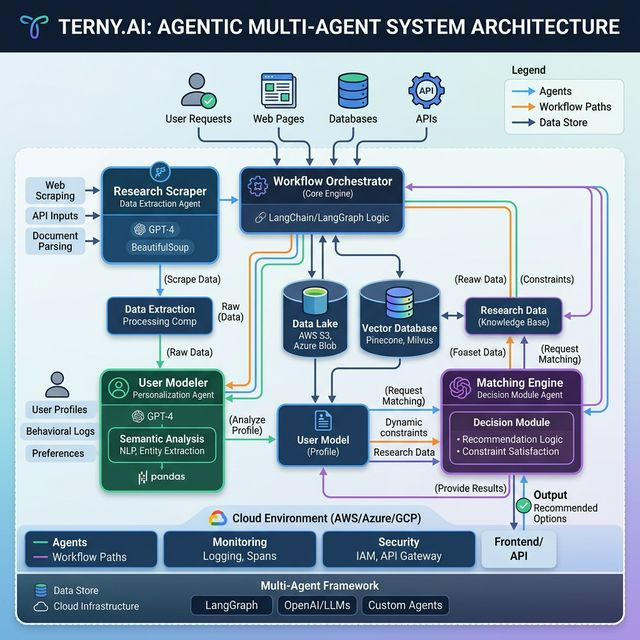
\includegraphics[width=0.85\textwidth]{agent_architecture.png}
    \caption{terny.ai 的多智能體協作與 RAG 決策流程圖}
\end{figure}

\newpage

\subsection{上海比特無限實習：工業指令意圖識別}

\subsubsection{任務描述}
針對 130+ 類複雜的工業指令（如機械設備控制指令），將自然語言精確轉換為系統可執行的意圖數據。

\subsubsection{關鍵突破：從 27\% 到 86\%}
這是我最具代表性的實戰成果。我採取的策略包括：
\begin{enumerate}
    \item \textbf{多維度 Prompt Engineering}：引入 Few-Shot 思維與 Chain-of-Thought（CoT），讓模型理解工業術語的上下文。
    \item \textbf{結構化驗收測試 (UAT)}：設計了一套自動化評分框架，能夠及時反饋模型在特定場景（如重疊意圖）下的表現。
    \item \textbf{VLM 文件審核}：使用視覺語言模型讀取掃描件，將數據提取精確到表格級別，使原本需 1 小時的人工錄入縮短至 5 分鐘。
\end{enumerate}

\subsubsection{技術細節與研發路徑}
\begin{itemize}
    \item \textbf{資料採集智能體}：針對 50+ 個高度非結構化的學術實驗室網站，我們設計了語義分片（Semantic Chunking）策略，確保 LLM 能在雜亂的 HTML 中精確提取出教授的「招募動向」。
    \item \textbf{LangGraph 決策迴圈}：解決了傳統 RAG 的「檢索失效」問題。如果初始檢索結果不理想，系統會自動生成新的檢索查詢（Query Rewriting）進行二次檢索。
    \item \textbf{跨語言統一 Embedding}：針對日本、歐盟與北美的實驗室資訊，我們調優了多語言向量模型，消弭了因語言翻譯差異導致的匹配偏差。
\end{itemize}

\newpage

\subsection{材料性質預測專案之深度技術解析}

針對 OC22/DFT 數據集的處理，我們並非僅套用現成模型，而是進行了底層的特徵設計。

\subsubsection{模型設計邏輯}
使用圖神經網絡 (GNN) 捕捉晶體結構的週期性特徵 (Periodicity)，並將其映射至多維向量空間。這一過程不僅僅是計算，更是對物理場的一種數值模擬。

\subsubsection{與 Lambton College 專案的關聯}
Lambton College 在先進材料與能源領域有深厚積累。我在處理材料數值模擬數據時累積的管道（Pipeline）處理經驗，將能無縫對接至 AURORA 專案中涉及材料資源優化的部分。這既是技術的遷移，也是學術領域的跨界整合。

\newpage

\newpage

\section{對所申請計畫與機構的深度理解}

\subsection{Lambton College：加拿大 R\&I 的領航者}

Lambton College 不僅是教學機構，更是加拿大排名第二的研究型學院。其在「生物、先進材料、能源」等領域的研發動能極強，這需要極高效的後勤與數據支持系統。

\subsection{FASTER 負責任 AI 框架與我的人性化技術觀}

Lambton College 提出的 \textbf{FASTER} 原則（Fairness, Accountability, Security, Transparency, Education, Relevance）令我倍感振奮。這與我在「專業倫理」課程中學到的理論產生了強烈共鳴：
\begin{itemize}
    \item \textbf{不僅是代碼，更是責任}：我曾在助教工作中親見算法偏見帶來的焦慮，因此我極度渴望學習該機構如何將「倫理」從口號轉化為開發流程中的 Checkpoint。
    \item \textbf{淋漓盡致的實踐}：我希望觀察該部門如何在追求 AURORA 效率的同時，依然能保證算法對所有合作夥伴與獎助金申請者的公平性。
\end{itemize}

\begin{figure}[h]
    \centering
    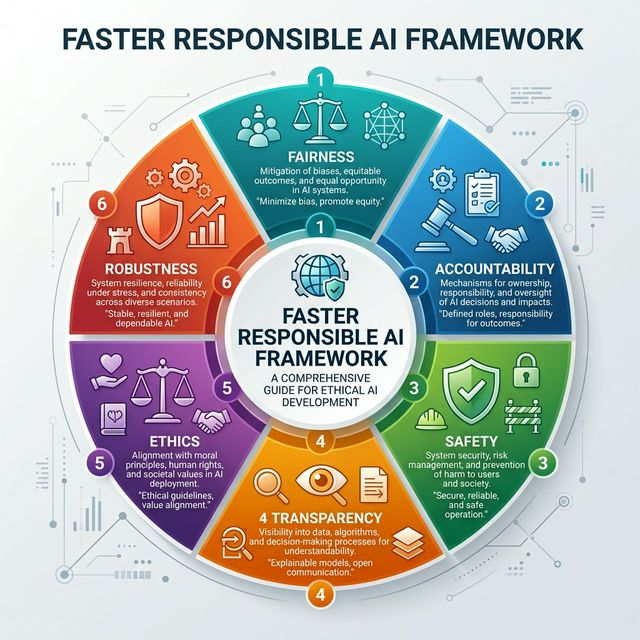
\includegraphics[width=0.6\textwidth]{faster_framework.png}
    \caption{FASTER Responsible AI 治理框架圖解}
\end{figure}

\subsection{AURORA 專案的技術目標}

AURORA-Biz 與 AURORA-Grants 的核心在於「匹配」。這正是我在 \texttt{terny.ai} 中深耕的領域。我能帶來的直接貢獻包括：
\begin{itemize}
    \item \textbf{高性能 RAG 檢索器}：處理龐大的研究資料庫與補助條款。
    \item \textbf{Multi-Agent 審核流}：自動校驗申請書內容是否符合特定的資助倫理條款。
\end{itemize}

\newpage

\section{計畫執行細節規劃 (14 週全圖表)}

本次為期 14 週的遠征將嚴格執行，每一週都設有明確的目標與可衡量的 KPI。

\subsection{細化的 14 週執行地圖 (Weekly Technical Roadmap)}

本章節將原本的階段性規劃進一步拆解為每週的具體執行指標與交付物。

\subsubsection{第一階段：基礎對接與環境調優}
\begin{itemize}
    \item \textbf{Week 1 (系統初始化)}：重點在於開發環境的權限配置。交付物：開發環境配置手冊、Git 同步測試報告。
    \item \textbf{Week 2 (理論與合規)}：深入研讀 Lambton College 的 R\&I 倫理指南，並撰寫一份「Ethics in AURORA」的內部備忘錄。
    \item \textbf{Week 3 (業務邏輯對齊)}：與 AURORA-Grants 的核心用戶進行 Deep Dive，識別出現有系統中 3 個最重要的效率瓶頸點。
\end{itemize}

\newpage

\subsubsection{第二階段：模型開發與 RAG 優化循環 (核心週期)}
\begin{itemize}
    \item \textbf{Week 4 (資料前處理)}：建立資料清洗管道，處理來自加拿大政府補助網站的非結構化數據。
    \item \textbf{Week 5 (RAG Baseline)}：部署首個向量資料庫（如 Pinecone 或 Weaviate），實現基礎關鍵字與語義搜索。
    \item \textbf{Week 6 (智能體邏輯構建)}：開始撰寫 \texttt{LangGraph} 節點邏輯，用於處理補助金申請書的初版自動校核。
    \item \textbf{Week 7 (特徵挖掘)}：提取合作夥伴的歷史成功因子，注入匹配模型中以提升媒合率。
    \item \textbf{Week 8 (深度調優)}：測試不同的 Open Models (如 Llama-3, Qwen) 在專業研究領域的摘要與比較性能。
    \item \textbf{Week 9 (效能基準)}：針對 500+ 本地測試用例運行數據觀測性測試，量化各節點的推理延遲。交付物：效能基準分析報告。
\end{itemize}

\newpage

\subsubsection{第三階段：部署集成與技術傳承}
\begin{itemize}
    \item \textbf{Week 10 (Azure 雲端集成)}：將功能模組遷移至雲端生產環境，測試端到端 (E2E) 的數據流動。
    \item \textbf{Week 11 (負責任 AI 審計)}：根據 FASTER 原則，進行偏見審核與壓力測試，確保輸出的夥伴建議不具備歧視性。
    \item \textbf{Week 12 (QA 與用戶測試)}：在測試環境中進行為期一週的 Beta 測試，收集 R\&I 部門員工的反饋。
    \item \textbf{Week 13 (文檔固化)}：撰寫開發者維運手冊、API 文檔以及面向普通用戶的操作手冊。
    \item \textbf{Week 14 (結案發表)}：向 Lambton College 研究副校長或 R\&I 部門主管進行成果展示，總結貢獻與未來展望。
\end{itemize}

\newpage

\newpage

\section{職涯地圖與回國後的社會貢獻}

\subsection{個人成長目標：從 AI 學生到 AI 工程師}

這次見習是我職涯的重要轉折點。我不僅要學習寫代碼，更要學習在一個加拿大頂尖研究體系中，如何系統性地進行「技術選型」與「技術治理」。

\subsection{5--10 年長期職涯規劃}
\begin{itemize}
    \item \textbf{短程 (1--2 年)}：在台大或交大完成研究生學業，並將 Lambton 的 R\&I 運作模式引入本地項目。
    \item \textbf{中程 (3--5 年)}：進入半導體或電子業的 AI 中心，專注於推動「工業自動化中的倫理 AI」。
    \item \textbf{長程 (5--10 年)}：成為具有國際影響力的 AI 系統架構師，致力於建設更具透明度與社會價值的智能基座。
\end{itemize}

\subsection{回國後的具體影響計畫}

\subsubsection{技術分享：Responsible AI 系列講座}
我將在校內舉辦至少兩場分享會，主題圍繞「如何在工業開發中嵌入 FASTER 倫理原則」，將加拿大的一手經驗傳承給更多學術同儕。

\subsubsection{EduNexus AI：構建下世代 AI 智能助教平台}

我計畫在學成返台後，結合交大助教經驗與見習所學，開發一個名為 **EduNexus AI** 的開源教育平台。其核心設計將包含三個技術層面：

\begin{enumerate}
    \item \textbf{動態知識圖譜層 (GNN-based Knowledge Mapping)}：
    針對我在多年家教中發現的「定位弱點」難題，我將運用 GNN 將課程概念建模。透過追蹤學生的歷史反應，AI 能如同經驗豐富的導師一般，迅速找出其「知識盲區」，實現真正的因材施教。
    
    \item \textbf{情境感應輔導層 (Context-Aware RAG Tutoring)}：
    基於 Lambton College 的 R\&I 實踐，EduNexus 將利用 RAG 技術對教材、講義進進行索引，確保 AI 助教的回答絕無幻覺（Hallucination），並能嚴格遵循教師的教學目標。
    
    \item \textbf{自動化行政代理 (Agentic Administrative workflows)}：
    將 n8n 的自動化思維深化為「多智能體工作流」。Agent 能自動處理發放作業、追蹤遲交情況並撰寫每週學習報告，讓教師能將精力集中在更高價值的啟發式教學上。
\end{enumerate}

這項計畫不僅是技術的展示，更是我將「AI 倫理」與「教育公平」落實於本土社會的具體實踐。我將邀請交大的學弟妹參與 Beta 測試，逐步推廣至全台高校。

\newpage

\section{經費需求與外語溝通能力}

\subsection{經費預算辦理方式}

本人已詳閱計畫經費標準，同意依據本計畫平台公布之標準依實報銷辦理。

\vspace{0.3cm}
$\boxtimes$ 同意編列方式

\subsection{外語溝通實力證明}

為了確保見習期間的技術溝通無礙，我具備以下外語優勢：
\begin{itemize}
    \item \textbf{英語 (核心溝通語)}：
    \begin{itemize}
        \item 具備全英文專業授課證書，CEFR B2/C1 等級實力。
        \item 在密西根學院累積 3 年技術寫作與簡報經驗，能流利使用英文討論模型架構與數據倫理。
    \end{itemize}
    \item \textbf{日語 (第二外語)}：
    \begin{itemize}
        \item 慶應義塾大學交換背景，具備日常工作生活流暢溝通能力。
    \end{itemize}
    \item \textbf{閩南語}：母語級別，利於回國後與基層場景進行技術普及溝通。
\end{itemize}

\newpage

\section*{附件：合作單位技術提問回答 (Extended English Annex)}

\subsection*{Q1: Explain a complex machine learning model architecture you implemented.}

\textbf{Implementation: GNN + Transformer for Material Science}

In my recent research project, I tackled the challenge of predicting atomic properties using the \textbf{OC22 dataset}. Traditional Graph Neural Networks (GNNs) excel at capturing local atomic geometries, but often struggle with long-range interactions across a lattice structure. 

To address this, I implemented a hybrid architecture:
\begin{itemize}
    \item \textbf{Graph Convolutional Layers}: Used to extract local features by treating atoms as nodes and chemical bonds as edges.
    \item \textbf{Transformer Layers}: Applied on top of the node embeddings to allow "all-to-all" attention, enabling the model to learn synergistic relationships between distant atoms.
    \item \textbf{Result}: This hybrid approach achieved a significant reduction in Mean Squared Error (MSE) compared to vanilla GNN models, demonstrating the power of combining structural priors with global attention mechanisms.
\end{itemize}

\subsection*{Q2: Choosing between LLM frameworks (LangChain vs. LangGraph).}

\textbf{Reflection: Why I chose LangGraph for terny.ai}

While \textbf{LangChain} is excellent for rapid prototyping of linear chains, I found it insufficient for \texttt{terny.ai}, which requires cyclic reasoning (e.g., searching for info, evaluating its relevance, and deciding whether to re-search or stop).

\textbf{LangGraph} provides:
\begin{enumerate}
    \item \textbf{State Persistence}: Allowing the system to "remember" why it failed a previous search.
    \item \textbf{Cyclic Flows}: Supporting loops and iterative refinement which are essential for high-accuracy RAG.
    \item \textbf{Control}: Giving me precise control over which agent (node) communicates with which, significantly reducing hallucinations.
\end{enumerate}

\subsection*{Q3: The role of "Data Observability" in your current internship.}

At BitUnlimited, I realized that a model is only as good as its input observability. I built a \textbf{Performance Dashboard} that tracks not just the final accuracy (which jumped to 86\%), but also:
\begin{itemize}
    \item \textbf{Token Latency}: Identifying which specific nodes in our pipeline were bottlenecks.
    \item \textbf{Intent Drif}: Monitoring if the user's natural language patterns were shifting away from our training set.
    \item \textbf{Faithfulness}: Using AI judges to ensure the LLM's outputs were strictly grounded in the industrial documentation.
\end{itemize}

\subsection*{Q4: How do you handle technical ambiguity and team conflicts?}

When project requirements are ambiguous (as they often are in AI), I apply the **"First Principles"** approach:
\begin{enumerate}
    \item \textbf{Define the MVP}: Anchor the team on the smallest verifiable success metric.
    \item \textbf{Shorten the Feedback Loop}: In team settings, I promote "daily stand-ups" or technical syncs to resolve misunderstandings before they turn into code-level conflicts.
    \item \textbf{Documentation as Truth}: I use detailed documentation (like the ones I am proposing here) to ensure every team member is aligned with the latest architecture decisions.
\end{enumerate}

\end{document}